% Source PDF page 395 (printed p. 381)
这个问题有一个有趣的几何解释。它等价于
\[
\begin{array}{ll}
\text{最小化}&b^{\T}u+(1/2)\norm{A^{\T}u}_2^2\\
\text{满足}&u\succeq0,
\end{array}
\]
而后者是
\[
\begin{array}{ll}
\text{最大化}&-(1/2)\norm x_2^2\\
\text{满足}&Ax\preceq b
\end{array}
\]
的对偶。换言之，Chernoff界为
\begin{equation}
 \Prob(X\in C)\le\exp(-\dist(0,C)^2/2),\tag{7.22}
\end{equation}
其中 $\dist(0,C)$ 是原点到 $C$ 的欧几里得距离。

\begin{quote}\textbf{说明7.3}
不用Chernoff不等式，也能推导界（7.22）。若原点到 $C$ 的距离为 $d$，则存在包含 $C$ 的半空间 $H=\{z\mid a^{\T}z\ge d\}$，且 $\norm a_2=1$。随机变量 $a^{\T}X$ 服从 $N(0,1)$，因此
\[
 \Prob(X\in C)\le\Prob(X\in H)=\Phi(-d),
\]
其中 $\Phi$ 是零均值、单位方差高斯分布的累计分布函数。由于 $d\ge0$ 时 $\Phi(-d)\le e^{-d^2/2}$，这个界至少与Chernoff界（7.22）一样紧。
\end{quote}

\subsection{例子}
本节用一个检测例子说明Chebyshev与Chernoff概率界方法。有一组 $m$ 个可能符号或信号 $s\in\{s_1,s_2,\ldots,s_m\}\subseteq\R^n$，称为\emph{信号星座}。其中一个信号通过有噪声信道发送，接收信号为 $x=s+v$，其中噪声 $v$ 建模为随机变量。假设 $\E v=0$、$\E vv^{\T}=\sigma^2I$，即噪声分量 $v_1,\ldots,v_n$ 零均值、不相关，且方差均为 $\sigma^2$。接收机必须根据 $x=s+v$ 估计发送了哪个信号。\emph{最小距离检测器}选择与 $x$ 欧几里得距离最近的符号 $s_k$ 作为估计。如果 $v$ 高斯，则最小距离解码与最大似然解码相同。

若发送 $s_k$，给定 $x$ 时估计仍为 $s_k$，就正确检测。它发生在 $x$ 比起其他信号更接近 $s_k$ 时，即
\[
 \norm{x-s_k}_2<\norm{x-s_j}_2,\qquad j\ne k.
\]
因此，噪声 $v$ 满足以下线性不等式时，正确检测符号 $s_k$：
\[
 2(s_j-s_k)^{\T}(s_k+v)<\norm{s_j}_2^2-\norm{s_k}_2^2,
 \qquad j\ne k.
\]
这些不等式定义信号星座中 $s_k$ 的Voronoi区域 $V_k$，即比起星座中其他信号更接近 $s_k$ 的点集。正确检测 $s_k$ 的概率为 $\Prob(s_k+v\in V_k)$。图7.5给出 $m=7$、$n=2$ 的简单例子。

% Source PDF page 396 (printed p. 382)
\begin{figure}[htbp]\centering
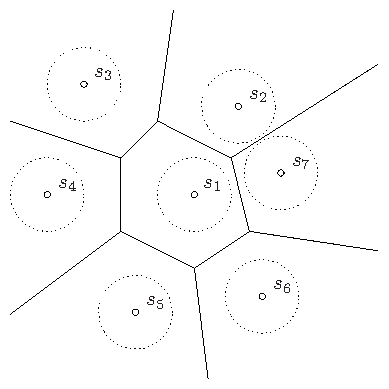
\includegraphics[width=.70\textwidth]{figures/ch07-figure-5.pdf}
\caption*{图7.5\quad 七个信号 $s_1,\ldots,s_7\in\R^2$ 构成的星座，以小圆圈表示。线段给出相应Voronoi区域的边界。当接收信号比起其他点更接近 $s_k$ 时，即位于 $s_k$ 的Voronoi区域内部时，最小距离检测器选择符号 $s_k$。每个点周围的大圆半径为一，用于展示尺度。}
\end{figure}

\subsubsection*{Chebyshev界}
半正定规划界（7.19）给出正确检测概率的下界。图7.6画出对 $s_1,s_2,s_3$ 三个符号，这些下界随噪声标准差 $\sigma$ 的变化。它们适用于任意零均值、协方差为 $\sigma^2I$ 的噪声分布。这些界是紧的，含义是：存在一个零均值、协方差 $\Sigma=\sigma^2I$ 的噪声分布，使错误概率等于该下界。图7.7给出第一个Voronoi集合、$\sigma=1$ 时的情形。

\subsubsection*{Chernoff界}
用同一例子说明Chernoff界。此时假设噪声高斯，即 $v\sim N(0,\sigma^2I)$。若发送符号 $s_k$，正确检测概率为 $\Prob(s_k+v\in V_k)$。为求该概率的下界，用二次规划（7.21）计算ML检测器选择符号 $i$ 的概率上界，$i=1,\ldots,m$、$i\ne k$。这些上界分别与 $s_k$ 到Voronoi集 $V_i$ 的距离有关。把将 $s_k$ 误作 $s_i$ 的各概率上界相加，得到错误概率上界，进而得到正确检测 $s_k$ 的概率下界。图7.8给出 $s_1$ 的下界，以及由Monte Carlo分析获得的正确检测概率估计。

% Source PDF page 397 (printed p. 383)
\begin{figure}[htbp]\centering
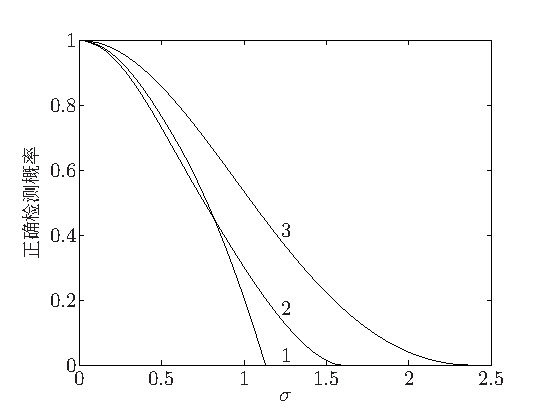
\includegraphics[width=.70\textwidth]{figures/ch07-figure-6.pdf}
\caption*{图7.6\quad 符号 $s_1,s_2,s_3$ 正确检测概率的Chebyshev下界。对所有零均值、协方差为 $\sigma^2I$ 的噪声分布，这些界都成立。}
\end{figure}
\begin{figure}[htbp]\centering
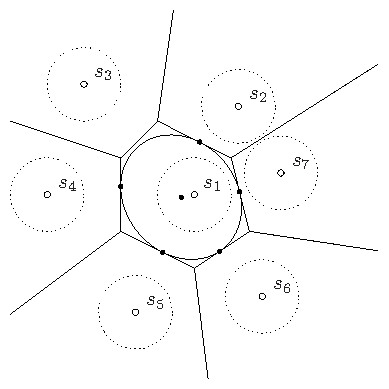
\includegraphics[width=.70\textwidth]{figures/ch07-figure-7.pdf}
\caption*{图7.7\quad $\sigma=1$ 时，正确检测符号1的概率的Chebyshev下界为0.2048，图示离散分布取到这一界。实心圆为接收信号 $s_1+v$ 的可能值。椭圆中心处的点概率为0.2048，边界上五个点的总概率为0.7952。椭圆由 $x^{\T}Px+2q^{\T}x+r=1$ 定义，其中 $P,q,r$ 为半正定规划（7.19）的最优解。}
\end{figure}

% Source PDF page 398 (printed p. 384)
\begin{figure}[htbp]\centering
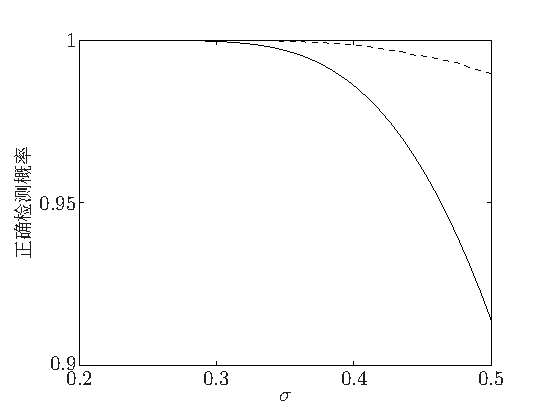
\includegraphics[width=.70\textwidth]{figures/ch07-figure-8.pdf}
\caption*{图7.8\quad 正确检测符号 $s_1$ 的概率随 $\sigma$ 变化的Chernoff下界（实线）和Monte Carlo估计（虚线）。本例噪声为零均值、协方差 $\sigma^2I$ 的高斯噪声。}
\end{figure}

\section{实验设计}
考虑根据测量或实验
\[
 y_i=a_i^{\T}x+w_i,\qquad i=1,\ldots,m
\]
估计向量 $x\in\R^n$，其中 $w_i$ 是测量噪声。假设 $w_i$ 是相互独立、零均值、单位方差的高斯随机变量，测量向量 $a_1,\ldots,a_m$ 张成 $\R^n$。$x$ 的最大似然估计与最小方差估计相同，均为最小二乘解
\[
 \widehat x=\left(\sum_{i=1}^ma_ia_i^{\T}\right)^{-1}
 \sum_{i=1}^my_ia_i.
\]
相应估计误差 $e=\widehat x-x$ 的均值为零，协方差矩阵为
\[
 E=\E ee^{\T}=\left(\sum_{i=1}^ma_ia_i^{\T}\right)^{-1}.
\]
矩阵 $E$ 刻画估计精度，或实验所提供的信息量。例如，$x$ 的 $\alpha$ 置信水平椭球为
\[
 \mathcal E=\{z\mid(z-\widehat x)^{\T}E^{-1}(z-\widehat x)\le\beta\},
\]
其中常数 $\beta$ 依赖于 $n,\alpha$。

假设表征测量的向量 $a_1,\ldots,a_m$，可以从 $p$ 个可能测试向量 $v_1,\ldots,v_p\in\R^n$ 中选择，即每个 $a_i$ 都是某个 $v_j$。

% Source PDF page 399 (printed p. 385)
\emph{实验设计}的目标是从可能向量中选择 $a_i$，使误差协方差 $E$ 在某种意义下尽量小。换言之，$m$ 次实验或测量中的每一次，都从固定的 $p$ 种可能实验中选择；任务是找到一组联合起来信息量最大的测量。

用 $m_j$ 表示选择 $a_i=v_j$ 的实验次数，有
\[
 m_1+\cdots+m_p=m.
\]
误差协方差矩阵可表示为
\[
 E=\left(\sum_{i=1}^ma_ia_i^{\T}\right)^{-1}
 =\left(\sum_{j=1}^pm_jv_jv_j^{\T}\right)^{-1}.
\]
这表明误差协方差只依赖于每类实验所选择的次数，即 $m_1,\ldots,m_p$。

基本实验设计问题如下：给定可能实验的选项 $v_1,\ldots,v_p$ 和要进行的总实验次数 $m$，选择每类实验的次数 $m_1,\ldots,m_p$，使误差协方差 $E$ 在某种意义下尽量小。变量 $m_1,\ldots,m_p$ 当然必须为整数，并且总和等于给定实验总次数 $m$。得到优化问题
\begin{equation}
\begin{array}{ll}
\text{最小化（关于 }\mathbf S_+^n\text{）}
 &\displaystyle E=\left(\sum_{j=1}^pm_jv_jv_j^{\T}\right)^{-1}\\[4pt]
\text{满足}&m_i\ge0,\quad m_1+\cdots+m_p=m,\\
&m_i\in\Z,
\end{array}\tag{7.23}
\end{equation}
变量为整数 $m_1,\ldots,m_p$。

基本实验设计问题（7.23）是半正定锥上的向量优化问题。如果一种设计得到 $E$，另一种得到 $\widetilde E$，且 $E\preceq\widetilde E$，那么第一种设计肯定不比第二种差。例如，把置信椭球平移到原点以便比较时，第一种设计的置信椭球包含在第二种之中。还可以说，对任意向量 $q$，第一种设计对 $q^{\T}x$ 的估计都更好，即方差更低，因为两种设计下 $q^{\T}x$ 估计的方差分别为 $q^{\T}Eq$ 和 $q^{\T}\widetilde Eq$。下面将介绍几种常见标量化形式。

\subsection{松弛的实验设计问题}
当总实验次数 $m$ 与 $p$ 相当时，（7.23）可能是困难的组合问题，因为此时各 $m_i$ 都是小整数。但当 $m$ 远大于 $p$ 时，通过忽略或松弛 $m_i$ 的整数约束，可找到（7.23）的良好近似解。令 $\lambda_i=m_i/m$，表示 $a_j=v_i$ 的实验占总实验次数的比例，或第 $i$ 类实验的相对频率。

% Source PDF page 400 (printed p. 386)
用 $\lambda_i$ 可将误差协方差表示为
\begin{equation}
 E=\frac1m\left(\sum_{i=1}^p\lambda_iv_iv_i^{\T}\right)^{-1}.\tag{7.24}
\end{equation}
向量 $\lambda\in\R^p$ 满足 $\lambda\succeq0$、$\one^{\T}\lambda=1$，且每个 $\lambda_i$ 都是 $1/m$ 的整数倍。忽略最后这一约束，就得到问题
\begin{equation}
\begin{array}{ll}
\text{最小化（关于 }\mathbf S_+^n\text{）}
 &\displaystyle E=\frac1m\left(\sum_{i=1}^p\lambda_iv_iv_i^{\T}\right)^{-1}\\[4pt]
\text{满足}&\lambda\succeq0,\quad\one^{\T}\lambda=1,
\end{array}\tag{7.25}
\end{equation}
变量为 $\lambda\in\R^p$。为区别于原来的组合实验设计问题（7.23），称其为\emph{松弛的实验设计问题}。由于目标 $E$ 是 $\lambda$ 的 $\mathbf S_+^n$ 凸函数，（7.25）是凸优化问题。

组合实验设计问题（7.23）与松弛问题（7.25）之间有以下联系。显然，组合问题多了一个约束，因此松弛问题的最优值为组合问题的最优值提供下界。由松弛解可按以下方式构造组合问题的一个次优解。先简单舍入：
\[
 m_i=\operatorname{round}(m\lambda_i),\qquad i=1,\ldots,p.
\]
对应这一选择的向量 $\widetilde\lambda$ 为
\[
 \widetilde\lambda_i=(1/m)\operatorname{round}(m\lambda_i),\qquad i=1,\ldots,p.
\]
$\widetilde\lambda$ 每个分量都是 $1/m$ 的整数倍。显然，$\abs{\lambda_i-\widetilde\lambda_i}\le1/(2m)$，所以当 $m$ 大时，$\lambda\approx\widetilde\lambda$。这意味着约束 $\one^{\T}\widetilde\lambda=1$ 在 $m$ 很大时近似满足，也意味着两者相应的误差协方差矩阵接近。

松弛问题（7.25）还有另一种解释：把 $\lambda\in\R^p$ 看作实验 $v_1,\ldots,v_p$ 上的概率分布。选择 $\lambda$ 对应一个随机实验：每次实验 $a_i$ 以概率 $\lambda_j$ 取 $v_j$。

本节余下只讨论松弛的实验设计问题，因此省略“松弛”这一修饰。

\subsection{标量化}
对于半正定锥上的向量优化问题（7.25），人们提出了几种标量化方式。

% Source PDF page 401 (printed p. 387)
\subsubsection*{D最优设计}
使用最广泛的标量化称为\emph{D最优设计}，它最小化误差协方差矩阵 $E$ 的行列式，对应于在置信水平固定时，最小化所得置信椭球的体积。忽略 $E$ 中常数因子 $1/m$，再对目标取对数，问题可写成
\begin{equation}
\begin{array}{ll}
\text{最小化}&\displaystyle\log\det\left(\sum_{i=1}^p\lambda_iv_iv_i^{\T}\right)^{-1}\\[4pt]
\text{满足}&\lambda\succeq0,\quad\one^{\T}\lambda=1,
\end{array}\tag{7.26}
\end{equation}
它是凸优化问题。

\subsubsection*{E最优设计}
\emph{E最优设计}最小化误差协方差矩阵的范数，即 $E$ 的最大特征值。置信椭球 $\mathcal E$ 的直径，也就是最长半轴的两倍，正比于 $\norm E_2^{1/2}$，所以最小化 $\norm E_2$，在几何上相当于最小化置信椭球直径。E最优设计也可解释为，在所有 $\norm q_2=1$ 的 $q$ 中，使 $q^{\T}e$ 的最大方差最小。E最优实验设计问题为
\[
\begin{array}{ll}
\text{最小化}&\displaystyle\left\|\left(\sum_{i=1}^p\lambda_iv_iv_i^{\T}\right)^{-1}\right\|_2\\[4pt]
\text{满足}&\lambda\succeq0,\quad\one^{\T}\lambda=1.
\end{array}
\]
目标关于 $\lambda$ 凸，因此该问题凸。

E最优设计也可写成半正定规划
\begin{equation}
\begin{array}{ll}
\text{最大化}&t\\
\text{满足}&\displaystyle\sum_{i=1}^p\lambda_iv_iv_i^{\T}\succeq tI,\\
&\lambda\succeq0,\quad\one^{\T}\lambda=1,
\end{array}\tag{7.27}
\end{equation}
变量为 $\lambda\in\R^p$、$t\in\R$。

\subsubsection*{A最优设计}
\emph{A最优实验设计}最小化协方差矩阵的迹 $\tr E$。该目标就是误差范数平方的均值：
\[
 \E\norm e_2^2=\E\tr(ee^{\T})=\tr E.
\]
A最优实验设计问题为
\begin{equation}
\begin{array}{ll}
\text{最小化}&\displaystyle\tr\left(\sum_{i=1}^p\lambda_iv_iv_i^{\T}\right)^{-1}\\[4pt]
\text{满足}&\lambda\succeq0,\quad\one^{\T}\lambda=1.
\end{array}\tag{7.28}
\end{equation}
这同样是凸问题，也能像E最优设计那样写成半正定规划：
\[
\begin{array}{ll}
\text{最小化}&\one^{\T}u\\[3pt]
\text{满足}&\displaystyle\begin{bmatrix}
 \sum_{i=1}^p\lambda_iv_iv_i^{\T}&e_k\\e_k^{\T}&u_k
 \end{bmatrix}\succeq0,\quad k=1,\ldots,n,\\[4pt]
&\lambda\succeq0,\quad\one^{\T}\lambda=1,
\end{array}
\]

% Source PDF page 402 (printed p. 388)
变量为 $u\in\R^n$ 和 $\lambda\in\R^p$，$e_k$ 为第 $k$ 个单位向量。

\subsubsection*{最优实验设计与对偶性}
三种标量化问题的拉格朗日对偶具有有趣的几何意义。

D最优实验设计（7.26）的对偶可写为
\[
\begin{array}{ll}
\text{最大化}&\log\det W+n\log n\\
\text{满足}&v_i^{\T}Wv_i\le1,\quad i=1,\ldots,p,
\end{array}
\]
变量为 $W\in\mathbf S^n$，定义域为 $\mathbf S_{++}^n$，见习题5.10。这个对偶问题有简单解释：最优解 $W^\star$ 确定包含 $v_1,\ldots,v_p$、以原点为中心的最小体积椭球 $\{x\mid x^{\T}W^\star x\le1\}$，另见第222页问题（5.14）的讨论。由互补松弛，
\begin{equation}
 \lambda_i^\star(1-v_i^{\T}W^\star v_i)=0,\qquad i=1,\ldots,p,\tag{7.29}
\end{equation}
即最优设计仅使用位于该最小体积椭球表面上的实验 $v_i$。

E最优与A最优设计的对偶也有类似解释。问题（7.27）、（7.28）的对偶分别可写成
\begin{equation}
\begin{array}{ll}
\text{最大化}&\tr W\\
\text{满足}&v_i^{\T}Wv_i\le1,\quad i=1,\ldots,p,\\
&W\succeq0,
\end{array}\tag{7.30}
\end{equation}
以及
\begin{equation}
\begin{array}{ll}
\text{最大化}&(\tr W^{1/2})^2\\
\text{满足}&v_i^{\T}Wv_i\le1,\quad i=1,\ldots,p.
\end{array}\tag{7.31}
\end{equation}
两者的变量均为 $W\in\mathbf S^n$，第二个问题还有隐式约束 $W\in\mathbf S_+^n$，见习题5.40与5.10。

与D最优设计一样，最优解 $W^\star$ 确定一个包含 $v_1,\ldots,v_p$ 的极小椭球 $\{x\mid x^{\T}W^\star x\le1\}$。此外，$W^\star$ 与 $\lambda^\star$ 满足互补松弛（7.29），即最优设计只使用位于 $W^\star$ 所定义椭球表面的实验 $v_i$。

\subsubsection*{实验设计例子}
考虑 $x\in\R^2$、$p=20$ 的问题。图7.9用圆圈表示20个候选测量向量 $a_i$，原点以叉号表示。D最优实验只有两个非零 $\lambda_i$，以实心圆标在图7.9中；E最优实验也只有两个非零 $\lambda_i$，见图7.10；A最优实验有三个非零 $\lambda_i$，见图7.11。图中还画出三个与对偶最优解 $W^\star$ 关联的椭球 $\{x\mid x^{\T}W^\star x\le1\}$。图7.12给出所得90\%置信椭球，以及对所有实验赋予等权 $\lambda_i=1/p$ 的“均匀”设计的置信椭球。
